\documentclass[jou, apacite, 11pt, longtable, floatsintext, notab]{apa6}
\usepackage{epsf, epsfig, amssymb, amsmath, apacite, xcolor,
  booktabs, colortbl, rotating, setspace, fancyhdr}
% \usepackage{endfloat}
\usepackage{float}
\restylefloat{table}

\setcounter{topnumber}{1}
\setcounter{bottomnumber}{1}
\setcounter{totalnumber}{1}

\title{\textbf{Enhanced visuomotor learning and
    generalization in expert surgeons}}

\shorttitle{Expert visuomotor learning}

\author{Christopher L. Hewitson$^{1,2}$, Matthew J.
  Crossley$^{1,2,3}$, David M. Kaplan$^{1,2,3}$}

\affiliation{
  $^1$Macquarie University \\
  $^2$Perception in Action Research Centre \\
  $^3$Centre for Elite Performance, Expertise \& Training} 

\keywords{Visuomotor adaptation; sensorimotor
  learning; generalization; experts; surgery; minimally
  invasive surgery}

\authornote{Correspondence: David M. Kaplan, david.kaplan@mq.edu.au}

% \note{
%   \footnotesize
%   \noindent C.L.H. and D.M.K. conceived and designed the
%   experiments. C.L.H. performed the experiments. C.L.H. and
%   M.J.C. analyzed the data. All authors wrote the paper and
%   edited the manuscript. \\

%   \vspace{3mm}
%   \noindent The authors declare no competing interests. \\

%   \vspace{3mm}
%   \noindent This work is supported by an Australian Research
%   Council Centre of Excellence for Cognition and its Disorders
%   Grant [CE11000102] (to D.M.K.) and a Macquarie University
%   Research Seeding Grant [81340492] (to D.M.K.). \\

%   \vspace{3mm}
% }

\abstract{ 
  Although human motor learning has been intensively studied
  for many decades, it remains unknown whether group
  differences are present in expert cohorts that must
  routinely cope with and learn new visuomotor mappings such
  as expert minimally invasive surgeons. We found that expert
  surgeons compensate for a visuomotor perturbation more
  rapidly and to a greater extent than naive controls.
  Modelling indicates that these differences in expert
  behavioural performance reflects greater trial-to-trial
  retention, as opposed to greater trial-to-trial learning
  rate. We also found that surgeons generalize to novel reach
  directions more broadly than controls, a result which was
  subsequently verified by our modelling. In general, our
  findings show that minimally invasive surgeons exhibit
  enhanced visuomotor learning and generalization.
}


\begin{document}
\maketitle

\section{Introduction}
Human motor learning has been intensively studied for many
decades\cite{shadmehr_2010, krakauer_2011}. However, it
remains unknown whether group differences are present in
expert cohorts that must routinely cope with and learn new
visuomotor mappings such as minimally invasive surgeons.

Laparoscopic or minimally invasive surgery (MIS) is rapidly
replacing traditional open surgery for many procedures due
to its major benefits for patients over conventional open
surgery including reductions in infection risks, recovery
times, scarring, and overall hospital stays
[3].
Despite
these advantages, the task environment in MIS places high
demands on surgeons, increasing the difficulty relative to
open surgery for both initial learning \cite{braga_2002} and
ongoing performance
[3],[5],[6].
Since laparoscopic
instruments are controlled through small insertion points in
the skin, instrument movements are often mirror-reversed and
counter-intuitive (e.g., leftward hand motion produces
rightward instrument tip motion, and vice versa). Because
surgeons receive visual feedback indirectly via a
laparoscopic camera that is in turn projected to a video
display, rather than through direct observation, they must
also contend with a range of visualization problems
including absent depth information, variable magnification,
and a restricted and frequently distorted (e.g., rotated)
field of view. These factors, which are often subsumed under
the general rubric of ``challenges for hand-eye
coordination''
[7],
also impose heavy computational demands
on the brain and likely contribute to the significant
increase in time to achieve proficiency in MIS compared to
open surgery
[8],[9].

A related and potentially deeper explanation for why MIS is
difficult to learn is that it requires complex sensorimotor
transformations
[10],[11]
-- that is, the conversion of
sensory inputs into appropriate motor commands
[12].
These
transformations are not trivial, and are known to introduce
errors even for simple goal-directed movements such as
pointing to a visible target
[13],[14].
Moreover, because
this sensory-to-motor mapping can and often does change
during MIS such as when the laparoscopic camera rotates
relative to the workspace or the fulcrum point of the
instrument shifts, the same motor commands will not always
lead to the same outcome. Consequently, surgeons must be
particularly adept at learning new visuomotor
transformations so they can maintain accurate and consistent
motor performance during a procedure despite these
fluctuations. To appreciate the inherent challenges
involved, one can imagine trying to use a computer mouse if
the mapping between mouse and cursor movement frequently and
unpredictably changed.

If MIS introduces challenges for learning appropriate
visuomotor transformations, this suggests that expert
surgeons, who have successfully overcome these challenges,
might perform better than naive controls in a standard
visuomotor adaptation task in which a novel mapping is
imposed between hand motion and the corresponding visual
feedback
[15],[16].
This is either because (1) they will
have spent much more time practicing compensating for
visuomotor perturbations, (2) they are inherently more adept
than most people at compensating for visuomotor
perturbations and this is part of what makes them good
surgeons in the first place, or (3) some combination of both
these factors. The current literature does not address the
plausibility of either of these possibilities. For instance,
it is unknown to what degree the basic neural and cognitive
processes that drive visuomotor adaptation are capable of
enhancements in learning and performance in the first place.
On the other hand, it has never been directly shown that
expert surgeons, or any other group with superior motor
skill, derive their skilled behavior from better visuomotor
adaptation ability. This is precisely the hypothesis we
sought to test in this study.

Furthermore, it is plausible to assume that a broader or
more efficient generalization of visuomotor motor skill is a
benefit to expert MIS surgeons. Firstly, Many expert
surgeons concurrently shift between open, minimally invasive
and robotic surgery in quick succession, all of which
require visuomotor mappings unique to the relative surgical
domain. Secondly the accurate estimation and tracking of
tissue density and deformation is important to navigation
and motion compensation, features that are perturbed given
the dynamic visual feedback afforded to the surgeon during
minimally invasive surgery (Mountney and Yang 2008).
Accordingly it is coherent to assume that broader and more
efficient generalization of visuomotor motor skill is a
benefit to expert MIS surgeons .

We predicted that expert minimally invasive surgeons would
compensate more rapidly and more completely for a visuomotor
perturbation and therefore experience smaller errors, and
would exhibit a wider pattern of spatial generalization
of their learning than naive controls in a standard
visuomotor adaptation task
[16,17].
Our results were
generally consistent with these hypotheses.

\section{Methods}
\subsection{Participants}
10 expert surgeons and 10 naive controls participated in the
study. All were right-hand dominant (LQ > 70) assessed using
the ten-item version of the Edinburgh Handedness Inventory
[18], with normal or corrected to normal vision and no
reported motor impairments. All experts (age 47+/-14 years; 9
males, 1 female) had completed greater than 100 procedures
(range: 150-22000) with an average of 2900 (SD: 6000)
procedures. Naïve controls ($23\pm3$ years; 4 males, 6 females)
were university undergraduates with no prior medical or
surgical training and limited video game use ($\leq 3$ hours per
week)
[19–21].
All participants gave informed consent to
participate and the experimental protocols were approved by
the [redacted for review] Human Research Ethics Committee.
Sample size was consistent with field-standard conventions
for visuomotor adaptation and generalization experiments
[17,22,23]
as well as recent studies investigating group
differences in visuomotor learning
[24].

\subsection{Experimental Apparatus}
A unimanual KINARM endpoint robot (BKIN Technologies,
Kingston, Ontario, Canada) was utilized in the experiments
for motion tracking and stimulus presentation (Fig 1a-c).
The KINARM has a single graspable manipulandum that permits
unrestricted 2D arm movement in the horizontal plane. A
projection-mirror system enables presentation of visual
stimuli that appear in this same plane. Subjects received
visual feedback about their hand position via a cursor
(solid white circle, 2.5 mm diameter) controlled in
real-time by moving the manipulandum. Mirror placement and
an opaque apron attached just below the subject’s chin
ensured that visual feedback from the real hand was not
available for the duration of the experiment.

\subsection{Experimental Procedure}
Participants were instructed to perform fast and accurate
point-to-point reaching movements with the dominant (right)
arm using cursor feedback, whenever it was available.
Subjects performed reaches from a start target located at
the center of the workspace to 11 different target locations
9 cm away from the start target and spaced $30\deg$ apart (Fig
1d) The start target was a solid red circle (5 mm diameter),
and each reach target was a solid green circle (5 mm
diameter). The appearance of the reach target served as the
go cue. Participants were positioned so that the starting
target was directly in front of their torso.

The experiment began with a familiarization phase of 33
reach trials (3 per target in pseudorandom order) with
veridical visual feedback provided throughout the reach.
After the familiarization phase, participants rested for 1
minute. The baseline phase consisted of 198 reach trials
across all 11 target directions (18 trials per target). For
2/3 of the reaches (132 trials), veridical cursor feedback
was provided throughout the trial. For the remaining 1/3 (66
trials), visual feedback was withheld. During no-feedback
trials, the cursor disappeared as soon as the hand left the
start target. During the return movement, cursor feedback
was not provided. However, to help guide the participant’s
hand back to the start target a green ring centered over the
start target appeared with a radius equal to the distance
between the hand and start target. Once the participant’s
hand was 1 cm from the start target the ring was removed and
cursor feedback reinstated. After the baseline phase,
participants rested for 1 minute. The adaptation phase
consisted of 110 reaches toward a single target positioned
at $0\deg$ in the frontal plane (straight ahead; see figure 1).
As the participant reached toward the target, cursor
feedback was rotated about the start target by $30\deg$ (CW or
CCW; counterbalanced between participants). For the cursor
to move directly toward the target, hand motion would need
to be directed $30\deg$ opposite to the direction of the cursor
rotation. Visual feedback was withheld for the duration of
the outward reach on all trials and was only provided when
the subject’s hand came within 1 cm of the start target
during the return movement
[23].
For 90\% of the trials,
visual feedback was provided at movement offset for 150 ms.
These trials were used for baseline correction of adaptation
data. For the remaining 10\% of the trials, no visual
feedback was provided during the reach or at the endpoint.
These were used to baseline correct generalization data. The
generalization phase consisted of 66 reaches to 1 of 11
target directions (10 untrained directions) presented in
pseudorandom order without visual feedback. No visuomotor
rotation was imposed during the generalization phase.

\subsection{Data Analysis and Models}
Movement kinematics including hand position and velocity
were recorded for all trials using BKIN’s Dexterit-E
experimental control and data acquisition software (BKIN
Technologies). Data was recorded at 200 Hz and logged in
Dexterit-E. Custom scripts for data processing were written
in MATLAB (R2013a). Data analysis was performed in JASP
(0.9.2) and Python (3.7.3). Model fitting was done in Python
(3.7.3) using the SciPy (1.4.1) library. A combined spatial-
and velocity-based criterion was used to determine movement
onset, movement offset, and corresponding reach endpoints
[25,26]. Movement onset was defined as the first point in
time at which the movement exceeded 5\% of peak velocity
after leaving the start target. Movement offset was
similarly defined as the first point in time at which the
movement dropped below 5\% of peak velocity after a minimum
reach of 9 cm from the start target in any radial direction,
and reach endpoints were defined as the x and y values at
movement offset. Trials that failed to satisfy the minimum
reach distance of 9 cm were not included in the analysis. In
total, 210 trials (5.1\%) across all experimental phases
were discarded from the control group and 162 trials (3.9\%)
were discarded in total from the expert group.

To quantify baseline motor performance, reaction time (RT;
reach target onset – movement onset), total movement time
(MT; movement offset – movement onset), peak velocity (PV),
and hand angle (HA; hand position at movement offset) were
measured on each trial during the baseline phase in which no
visuomotor perturbation was imposed. To investigate
adaptation and generalization performance, we focused on HA.
Group differences in these performance metrics were
initially compared using analysis of variance (ANOVA) and
Welch t-tests ($\alpha < 0.05$). The Holm–Bonferroni method was
used to correct for multiple comparisons
[27].
Adaptation
and generalization data for both experts and controls were
baseline corrected to remove any intrinsic biases in
individual reach patterns. For adaptation data, this was
done by subtracting each participant’s mean hand angle
measured during the trials of the baseline phase, where
visual-feedback was provided an movement offset, from their
mean hand angle measured during the adaptation phase. For
generalization data, the procedure was exactly the same
except that mean hand angle was subtracted from no-feedback
baseline trials. Learning rates were initially analyzed
using repeated-measures ANOVA and Welch t-tests.
Greenhouse-Geisser corrected values for ANOVAs are reported
in case sphericity was violated. The Holm–Bonferroni method
was used to correct for multiple comparisons
[27].
Spatial
generalization of learning to new target directions was
compared between experts and controls using
repeated-measures ANOVAs.

To more comprehensively understand our adaptation and
generalization results, we also fit our data to a standard
state-space model of motor adaptation (Thoroughman and
Shadmehr 2000; Cheng and Sabes 2006). Many dominant theories
of motor learning assume that sensorimotor adaptation
involves the establishment and/or modification of internal
representations (so-called internal models) that map desired
motor goals into the time series of motor commands needed
for execution (Wolpert et al. 1998). It is thought that
these internal models get updated in response to error so
that errors can be reduced from one trial to the next. A
simple state-space model is governed by the following
equations:
\begin{equation}
  \delta_{t} = x_{t} - r_{t}
  \label{eq_simple_err}
\end{equation}
\begin{equation}
  x_{t} = \beta x_{t-1} - \alpha \delta_{t-1}
  \label{eq_simple_x}
\end{equation}
Here, $r_t$ is the imposed rotation on trial $t$, $x_t$ is
the state of the system at time $t$, which corresponds to
the current estimate of the rotation, and $\delta$ is the
error experienced on trial $t$. Equation \ref{eq_simple_x}
describes how states are updated from trial to trial. Here,
$\beta \in [0,1]$ is a free parameter that
determines how much of the current state $x_t$ is carried
over from the previous state $x_{t-1}$. That is, the system
has a tendency to decay back to its baseline value (i.e.,
$x_{t=0}$), and $\beta$ determines the rate of this decay.
Because of this, $\beta$ is often referred to as the
\emph{retention rate} or, or alternatively, as the
\emph{forgetting rate} parameter. On the other hand, $\alpha
\in [0,1]$ is a free parameter that determines how much of
the current state changes to compensate for the last
experienced error (i.e., $\alpha$ is the \emph{learning
rate}).

% The parameter captures the tendency for the adapted
% response to decay towards baseline levels with each
% subsequent movement and accounts for the fact that
% adaptation typically plateaus short of perfect compensation
% for the perturbation (Vaswani et al. 2015).

Equations \ref{eq_simple_err} and \ref{eq_simple_x} describe
a model of how motor commands are computed to accomplish a
single motor goal (e.g., reach to the training target that
is directly in front of you). For such a model to generate
many different motor commands to accomplish many different
motor goals, it needs to be augmented with the ability to
maintain separate states for each motor goal (i.e., target
direction). This is accomplished as follows:
\begin{equation}
  \boldsymbol{x}_{t} = \beta \boldsymbol{x}_{t-1} -
  \alpha \delta_{t-1} \boldsymbol{G} \boldsymbol{s}_{t-1}
  \label{eq_context_x_2}
\end{equation}
Here, $\boldsymbol{x_{t}}$ is a $n \times 1$ vector of
states, where $n$ is the number of states and is equal to
the number of distinct motor goals, and $\boldsymbol{s_{t}}$
is a $n \times 1$ indicator vector used to signal which
state is active on trial $t$ (i.e., the motor goal that was
planned for):
\begin{equation}
  \boldsymbol{x}_{t} = \begin{bmatrix} x_1 \\ x_2 \\ \vdots \\ x_n \end{bmatrix},
  \boldsymbol{s}_{t} = \begin{bmatrix} i_1 \\ i_2 \\ \vdots \\ i_n \end{bmatrix},
  i_{j} = \begin{cases}
    1, &
    \text{for reach } j \\ 0, & \text{otherwise}
  \end{cases}
\end{equation}
The error term $\delta_{t-1}$ is computed as:
\begin{equation}
  \delta_{t} = \boldsymbol{x}^{T}_{t} \boldsymbol{s}_{t} - r_{t}
    \label{eq_context_err}
\end{equation}
where $\boldsymbol{x}^{T}_{t}$ indicates the transpose of
$\boldsymbol{x}_{t}$. Finally, $\boldsymbol{G}$ is a
generalization function that specifies how adaptation that
occurs in one state influences adaptation in the other
states. Since all reaches executed in our experiments are
the same length, and differ only by their angular starting
position, we will express $\boldsymbol{G}$ as a function of
the angular distance between the current target direction,
$\theta_{0}$, and every other target direction $\theta_{i}$.
Following a the literature (Brayanov et al. 2012; Poggio and
Bizzi 2004), we assume that the generalization of adaptation
falls of as a Gaussian with distance from the goal target,
$\theta_{0}$:
\begin{equation}
  \boldsymbol{G} = e^{\frac{-(\theta_{0} - \boldsymbol{\theta})^2}{2 \sigma}}
\end{equation}
where
\begin{equation}
\boldsymbol{\theta} = \begin{bmatrix} \theta_1 \\ \theta_2 \\ \vdots \\ \theta_n \end{bmatrix}
\end{equation}

In many cases, simple state-space models such as those
described above under-predict the rate of adaptation
observed immediately following the introduction of a
perturbation. In response to this, visuomotor adaptation is
commonly modelled as reflecting the combined contributions
from two different learning processes, one fast and one slow
(Smith et al. 2006; McDougle et al. 2016), as follows:
\begin{equation}
  \boldsymbol{x}_{f, t} = \beta_{f} \boldsymbol{x}_{f,
    t-1} - \alpha_{f} \delta_{t-1} \boldsymbol{G} \boldsymbol{s}_{t-1}
  \label{eq_dual_rate_dual_1}
\end{equation}
\begin{equation}
    \boldsymbol{x}_{s, t} = \beta_{s} \boldsymbol{x}_{s,
      t-1} - \alpha_{s} \delta_{t-1} \boldsymbol{G} \boldsymbol{s}_{t-1}
    \label{eq_dual_rate_dual_2}
\end{equation}
\begin{equation}
  \boldsymbol{x}_{t} = \boldsymbol{x}_{f, t} + \boldsymbol{x}_{s, t}
  \label{eq_dual_rate_dual_3}
\end{equation}
\begin{equation}
  \alpha_{f} > \alpha_{s}, \beta_{f} < \beta_{s}
  \label{eq_dual_rate_dual_4}
\end{equation}
Here, all terms are as they were for the simple one-state
model, with the subscript $f$ and $s$ denoting the fast and
slow system, respectively. Equations
\ref{eq_dual_rate_dual_3} and \ref{eq_dual_rate_dual_4}
express the constraints on the parameter values such that
learning in the fast system must be faster than learning in
the slow system, and that retention in the fast system must
be smaller than retention in the slow system. Put another
way, this ensures that the fast system is fast and labile,
while the slow system is slow and stable.

Some researchers have proposed that the slow system
corresponds to a truly implicit motor process, and the fast
system corresponds to a cognitive process such as an
explicit aiming strategy (McDougle et al. 2015). Further,
these two systems are purported to have different
generalization functions (Heuer and Hegele 2011), (McDougle
et al. 2017). Further, these two systems are purported to
have difference generalization functions. In line with the
data suggesting this, we propose that $\boldsymbol{G}_{s}$
is defined as a Gaussian as previously described, but that
$\boldsymbol{G}_{f}$ is defined as a uniform shift:
\begin{equation}
  f(\theta) = C
\end{equation}
where $C$ is a scalar free parameter.

Our experiment includes three phases (i.e., baseline,
training, and generalization), and the context of each of
these phases may appear quite different to participants. For
example, during baseline, reaches are made and feedback is
given to all targets. During training, reaches are only made
to the training target. During generalization, reaches are
again made to all targets, but feedback is withheld. Because
of these context differences, it is possible that only a
portion of the adaptation acquired during the training phase
will transfer to the generalization phase (e.g., as is the
case in studies of inter-limb transfer of visuomotor
adaptation, where the context shift corresponds to switching
hands). To allow for this possibility we assume (where the
transfer between training and generalization occurs on trial
$t=306$):
\begin{equation}
  \boldsymbol{x}_{f, t=306} = \gamma_{f} \boldsymbol{x}_{f, t=306} 
\end{equation}
\begin{equation}
  \boldsymbol{x}_{s, t=306} = \gamma_{s} \boldsymbol{x}_{s, t=306} 
\end{equation}
Where $\gamma_{f} \in [0,1]$ and $\gamma_{s} \in [0,1]$ are
scalar free parameters. 

We fit this state-space model to the trial-by-trial endpoint
hand angles observed in the reported experiments, and used
the parameter estimates from the best-fitting model as
dependent measures. The model is fully specified by
equations \ref{eq_dual_rate_dual_1},
\ref{eq_dual_rate_dual_2}, \ref{eq_dual_rate_dual_3}, and
\ref{eq_dual_rate_dual_4}. The behaviour of the model is
fully characterised by eight parameters: two learning rates
($\alpha_s \in [0, 1]$ and $\alpha_f \in [0,1]$); two
retention rates ($\beta_s \in [0,1]$ and $\beta_f \in
[0,1]$), two generalization functions ($g_s \in [0, 150]$
and $g_f \in [0, 1]$), and the proportion of learning in
each system that transfers from training to generalization
($\gamma_s \in [0,1]$ and $\gamma_f \in [0,1]$).
We obtained best-fitting parameter estimates by minimising
the sum of squared error difference between the observed
endpoint hand angles and the model predictions:
\begin{equation}
  E = \sum_{t=1}^{N_{trials}} \left[ \boldsymbol{x}_{pred, t} - \boldsymbol{x}_{obs, t} \right]^2
  \label{eq_sse}
\end{equation}
To find the parameter values that achieved this minimum, we
used the differential evolution optimisation method
implemented in \textit{SciPy}. To construct 95\% confidence
intervals of the resulting parameter estimates, we created a
bootstrapped estimate of the sampling distributions of each
parameter. In particular, for each experiment and condition
containing $N$ participants, we sampled $N$
participants \textit{with replacement}, computed the average
endpoint hand angle per trial collapsing over subjects
(denoted by $\boldsymbol{x^{*}}$), and found the model
parameters that minimised the sum of squared error between
the model predictions and the bootstrap sample average:
\begin{equation}
    E^* = \sum_{t=1}^{N_{trials}} \left[ \boldsymbol{x}_{pred, t} - \boldsymbol{x^*}_{obs, t} \right]^2
  \label{eq_sse}
\end{equation}
We then repeated this procedure 10,000 times. 95\%
confidence intervals were constructed for each parameter
estimate by taking the 2.5 and 97.5 percentile values from
the bootstrap estimated sampling distribution.

\begin{figure}[t]
  \centering
  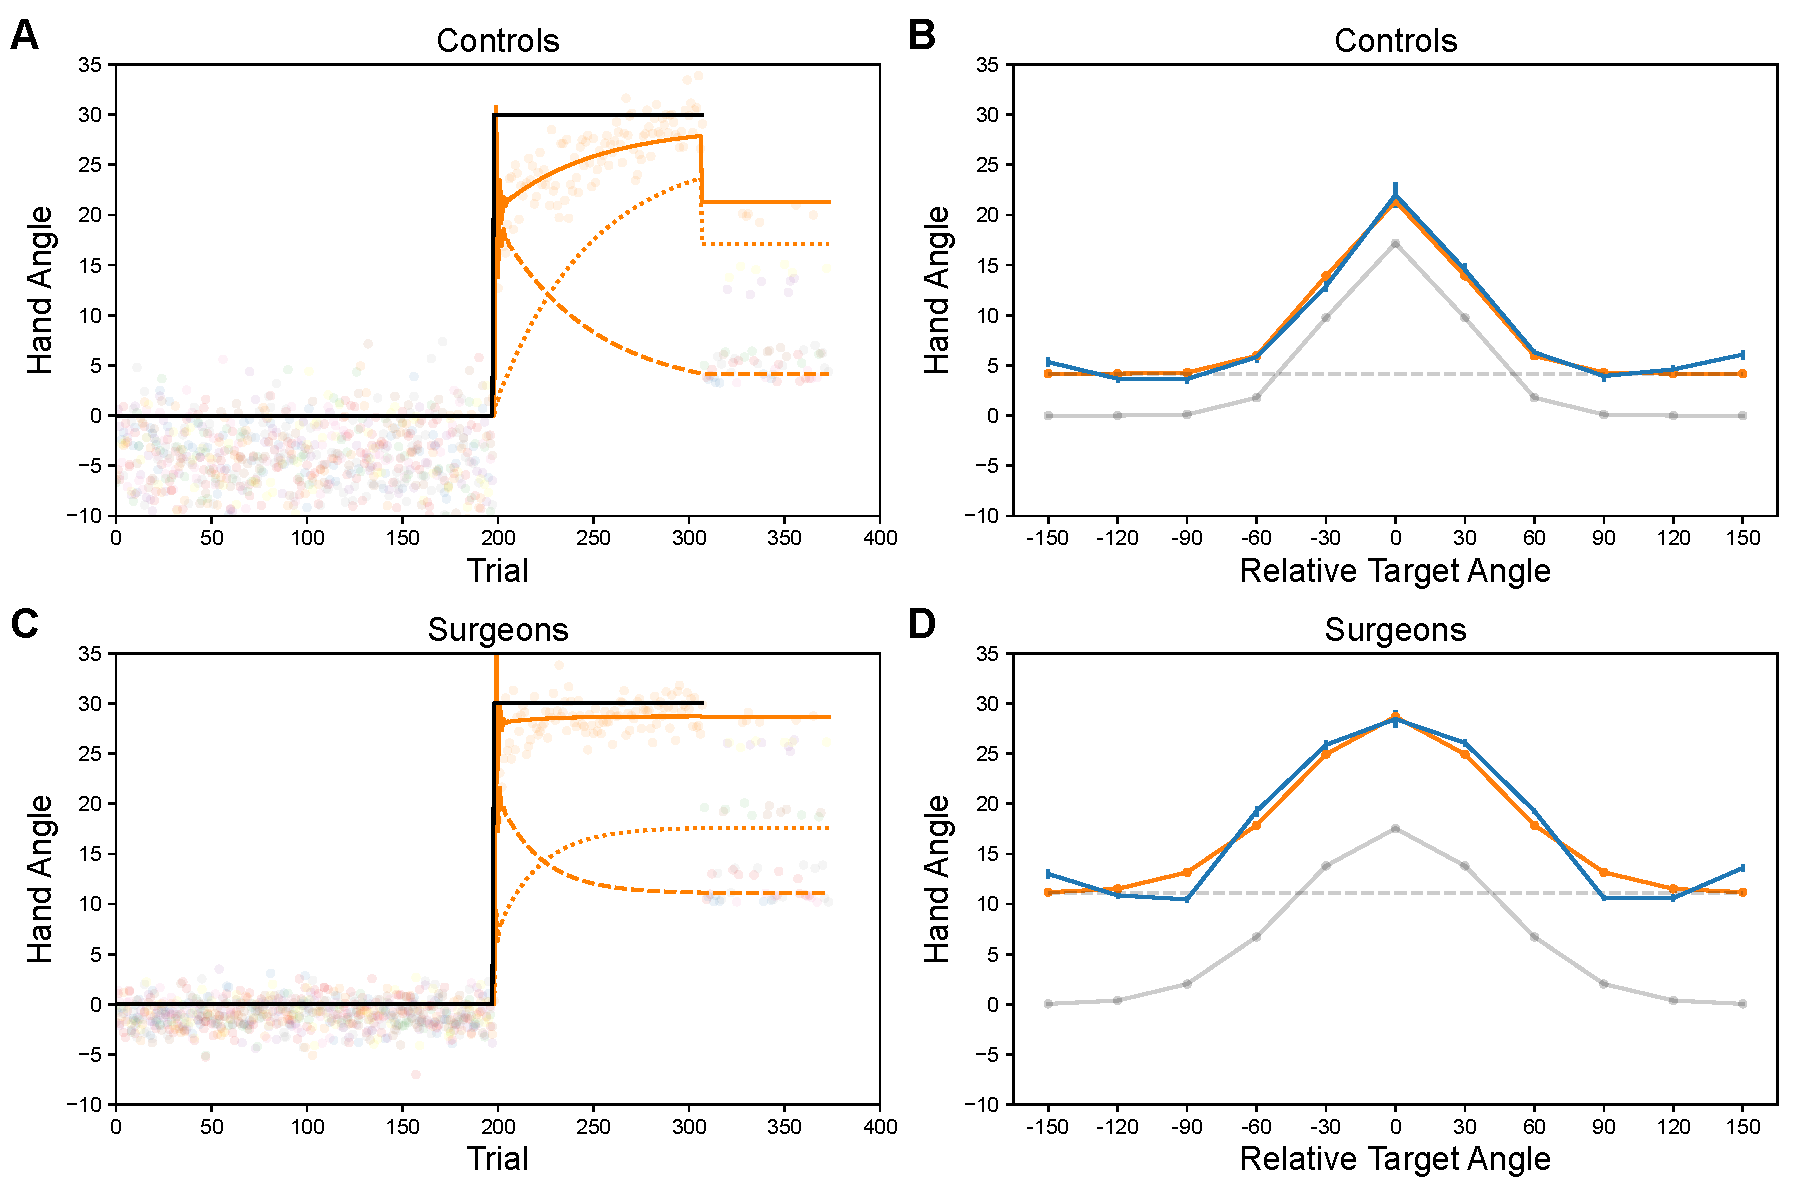
\includegraphics[width=0.5\textwidth]{figures/fig_results.pdf}
  \caption{\scriptsize
   \textbf{A:} Mean handle angles for controls.
   \textbf{B:} Generalization for controls.
   \textbf{C:} Mean hand angle for surgeons.
   \textbf{D:} Generalization for surgeons.
  }
  \label{fig_results}
\end{figure}
\section{Results}
Figure \ref{fig_results}A and \ref{fig_results}C show the
mean hand angle across all participants per group for each
trial of the experiment. Figure \ref{fig_results}B and
\ref{fig_results}D show the generalization pattern for each
group.

\subsection{Baseline motor performance}
First, we assessed group differences in baseline motor
performance. For all movement parameters (RT, MT, PV, HA),
we performed ANOVAs for the within-subject factors of TARGET
(11 target directions) and CONDITION (feedback vs
no-feedback), and the between-subject factor GROUP (experts
vs controls). While there was a significant effect of GROUP,
no GROUP $\times$ TARGET, or GROUP $\times$ TARGET $\times$
CONDITION interactions were observed indicating no
differences across target directions or feedback conditions
during the baseline phase (table \ref{table_1}).
\begin{table*}[t]
  \centering
  \footnotesize
  \begin{tabular}{ l|l|l|l } 
    & GROUP & GROUP $\times$ TARGET & GROUP $\times$ TARGET $\times$ CONDITION \\
    \hline
    RT & $F_{1,1}=331.1,  p_{h} <.001, \omega^2 = 0.077$ & $F_{1,1}0=1.218, p=.274$ & $F_{1,1}0=1.04, p_{h}>.99$\\ 
    MT & $F_{1,1} = 564, p_{h} <.001, \omega^2 = 0.124$ & $F_{1,1}0=1.137, p=.331$ & $F_{1,1}0=1.14, p_{h} >.99$\\ 
    PV & $F_{1,1} = 9.49, p_{h} =.002, \omega^2 = 0.002$ & $F_{1,1}0=0.91, p=.523$ & $F_{1,1}0=.384, p_{h} >.99$\\ 
    HA & $F_{1,1}=394.5, p_{h} <.001, \omega^2 = 0.091$ & $F_{1,1}0=0.752, p=.675$ & $F_{1,1}0=0.831, p_{h} >.99$\\
  \end{tabular}
  \label{table_1}
\end{table*}

Figure 2A and 2B show baseline reach trajectories for
representative subjects. Hand angles during baseline were
normally distributed (Shapiro-Wilk test; Controls baseline:
$p=.229$; Experts baseline: $p=.383$; Controls adaptation:
$p=.133$; Experts adaptation: $p=.208$). Experts were on
average more accurate. Error (rotation - hand angle) was
smaller for experts ($mean \pm SD = 1.1 \pm 2.4\deg$) than
for controls ($4.0\pm5.7\deg$) ($p<.001, d = 0.66$). Experts
were also more precise (exhibited lower variance) in their
movement endpoints compared to controls (INSERT STATS HERE).
RT was shorter on average ($350 \pm 180ms$) for experts than
for controls ($480 \pm 200ms$) ($p<.001, d = 0.61$), and MT
was shorter on average ($760 \pm 135ms$) for experts than
for controls ($900 \pm 180ms$)($p<.001, d= 0.795$). However,
peak velocity was greater for controls ($PV = 15.2\pm7.2
cm/s$) than experts ($14.4\pm6.5 cm/s$) ($p<.001, d =-
0.105$).

\subsection{Visuomotor adaptation}
We then tested whether the rate and extent of visuomotor
learning during the adaptation phase differed between
experts and controls. We performed a repeated measures ANOVA
on HA for the within-subject factor of BIN (10 trials per
bin), the interaction between BIN $\times$ GROUP, and the
between-subject factor of GROUP across 11 bins. There was a
significant within-subject effect of BIN ($F_{1,10} = 59.6,
p_h <.001, \omega^22 = 0.213$), which indicates that hand
angles in both groups changed over time in response to the
rotation. There was also a significant interaction between
BIN $\times$ GROUP ($F_{1,10} = 14.4, p_h <.001, \omega^2 =
0.058$), reflecting that experts compensated for the
rotation more quickly than controls. The effect size for
both comparisons was small. A significant between-subject
effect of GROUP ($F_{1,1} = 269, p_h <.001, \omega^2 =
0.573$), indicating an overall difference in hand angle
between groups. This effect size was more appreciable.

Group differences were present in the first two bins
(Experts adapted 73.7\% ($21.5 \pm 6.3 \deg$) compared to
62.9\% ($17.1 \pm 5.5 \deg$) for controls ($p<.001$;
baseline adjusted)), but not significant in the last two
bins (Experts adapted 98.7\% ($29.6 \pm 2.0\deg$) compared
to 94.9\% ($28.5 \pm 4.3\deg$) for controls ($p<.923$;
baseline adjusted)), indicating that experts differed from
controls initially, but that performance between the groups
ultimately reached similar asymptotic levels.

\subsection{generalization}
Finally, we investigated whether spatial generalization of
learning differed between the groups (Figure 3B and 3D show
the generalization pattern for each group). As with the
adaptation results, we first performed a repeated measures
ANOVA. The within-subject factor of TARGET and TARGET x
GROUP interaction, as well as the between-subject factor of
GROUP, were compared across the 11 targets (6 trials per
target). There was a significant within-subject effect of
TARGET ($F_{1,9.67} = 2518.2, p_h <.001, \omega^2 = 0.95$
Greenhouse-Geisser corrected) indicating that adaptation
generalized to different extents across target direction.
There was also a significant TARGET x GROUP interaction
($F_{1,9.67} = 130.8, p_h <.001, \omega^2 = 0.496$;
Greenhouse-Geisser corrected), indicating that experts
generalized more broadly than controls. The between-subject
effect of GROUP was also significant ($F_{1,1} = 12276, p_h
<.001, \omega^2 = 0.990$; Greenhouse-Geisser corrected),
indicating that experts’ pattern of generalization across
targets was different from controls.

\subsection{State-Space Modelling}
We also performed state-space modelling (see methods). The
predicted performance from the best fitting model is shown
in Figure 3. Figure \ref{fig_params} shows the best-fitting
value, along with the bootstrap estimated sampling
distributions for each model parameter.
\begin{figure}[h]
  \centering
  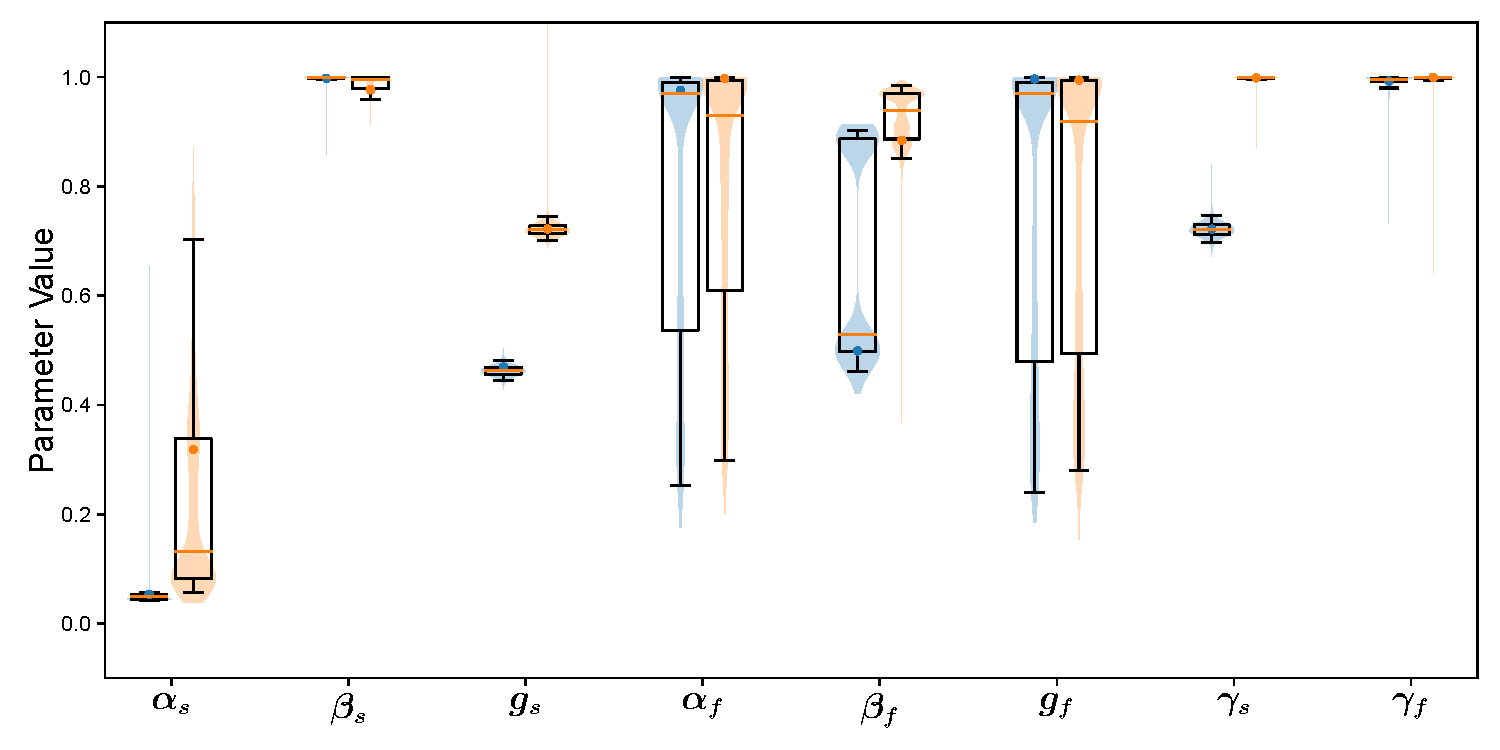
\includegraphics[width=0.5\textwidth]{figures/fig_params.pdf}
  \caption{\scriptsize
    Bootstrap estimated sampling distributions for every
    parameter in the fitted models.
  }
  \label{fig_params}
\end{figure}
For all statistical results reported below, we used a
bootstrap t-test (\cite{REFERENCE}). The difference in best
fitting parameter values between experts and controls was
significant for both retention parameters [$\beta_s: p<0.05;
\beta_f: p<0.01$], indicating that experts retained
trial-by-trial adaptation more than controls (i.e., experts
adapted -- in both fast and slow systems -- more stably than
controls). The slow system generalization width parameter
was also significantly different between groups [$g_s:
p<0.01$], indicating that experts generalized more broadly
than controls. Finally, the slow system context transfer
parameter was also significantly different between experts
and controls [$\gamma_s: p < 0.01$], reflecting that -- upon
transfer to the generalization phase -- experts retained
essentially all of their adaptation from training, whereas
controls lost a significant portion. Visual inspection of
Figure \ref{fig_results} shows that both experts and
controls display a positive uniform shift in their
generalization, and this is reflected in our best-fitting
$g_f$ values for these two groups, which are both
significantly different from zero (see Figure
\ref{fig_params}). However, the difference in this shift --
which appears greater for experts than for controls -- was
not statistically significant [$g_f: p=0.98$]. No other
between-group difference in parameters was significant
[$\alpha_s: p=0.09$; $\alpha_f: p=0.80$; $g_f: p=0.98$;
$\gamma_f: p=0.16$].

One of most interesting aspects of our data is that control
performance drops precipitously from the end of adaptation
to the generalization phase, and expert performance does not
(as reflected in the statistical difference in best-fitting
context transfer parameters $\gamma_s$). Inspection of
Figure \ref{fig_params} indicates that this difference must
be driven though the slow system, and shows that differences
in $\gamma_f$ cannot capture this results.

\section{Discussion}
In the current study, we hypothesized that expert minimally
invasive surgeons would exhibit enhanced visuomotor learning
compared to controls either because they draw on an
extensive body of experience coping with such visuomotor
perturbations, are inherently more adept at compensating for
visuomotor perturbations, or both. During minimally invasive
procedures an assistant typically directs the camera through
one of the ports on the opposite side of the patient to the
surgeon, and must often adjust the camera position and
orientation to improve the view of the operative field. This
means that the visual feedback the surgeon uses is often
rotated and/or translated. Importantly, every rotation and
translation of the camera is a visuomotor perturbation in
the sense that the mapping between surgical movements and
visual feedback is altered (i.e., the same motor commands
will not lead to the same visual outcome). These
considerations were the basis for our predictions about
enhanced visuomotor performance among expert surgeons.

Surprisingly little attention has been given to surgeons as
an informative expert cohort in visuomotor learning studies. More generally, there has been limited exploration of
group-level differences in visuomotor adaptation [24],[52].
In the most relevant study to date, Leukel and colleagues
[24] explored visuomotor learning in expert handball
players. Similar to our study, they reported lower
task-relevant movement variability (higher consistency) and
greater accuracy in their expert group prior to learning,
both widely considered to be hallmarks of expert performance
[53]. Yet interestingly, they observed no learning rate
differences in one experiment and a slower rate of
adaptation in experts compared to novices in another
experiment. One plausible explanation for this discrepancy
is that handball players do not have to contend with or
achieve mastery over changes in visuomotor mappings as do
expert surgeons with extensive training and experience
performing MIS. However, other differences between their
study and ours make precise comparisons difficult.

\subsection{State-space model is a process model}
Our analysis in this paper leans heavily on a two-state
state-space model that was  simultaneously fit to all phases
of our experimental data. Specifically, the fitting routine
was constrained to simultaneously find a single set of
parameters that best fit the pattern of reach endpoints
observed during baseline, adaptation, and generalization. In
other words, our state-space model is a process model for
how visuomotor adaptation and generalization might be
handled by the motor system, which sits somewhere in between
purely descriptive and mechanistic models (Dayan & Abbott
2001; Kaplan 2011). As such, our model departs from more
traditional curve-fitting approaches including fitting
exponential or power functions to adaptation data and
Gaussian functions to generalization data. It also differs
from state-space modelling approaches that fit only a subset
of data at a time (e.g., using one set of parameters to fit
adaptation and another to fit generalization).

\subsection{Group differences during adaptation are driven
  by retention rate and not learning rate}
In a standard visuomotor adaptation task, we found that
expert minimally invasive surgeons compensate for visuomotor
perturbations more rapidly than naive controls, but to an
equal extent. To shed light on possible drivers of this
effect, we developed a computational model that assumed that
visuomotor adaptation is driven through the combination of
two learning systems or processes -- one that is fast and
labile, and another that is slow and stable (Smith et al.
2006). This model explicates several factors that could make
experts compensate more successfully than controls, the most
intuitive of which is that experts adapt more in response to
experienced errors (i.e., experts might have a larger
learning rate then controls). Our modelling results reject
this hypothesis, although there was a trend in this
direction (e.g., a one-tailed test for $\alpha_s$ being
larger for experts than for controls was significant at
p<0.05). This suggests that there may in fact be real
learning differences between groups, but that our study may
have been under-powered.

Another possibility is that experts might exhibit more stable
adaptation than controls (i.e., they might have a larger
retention rate than controls). Our modelling results
strongly suggest that this is the case, but the exact
mechanism must be considered carefully. In particular,
relative to controls, experts had more stable adaptation in
the fast system, but less stable adaptation in the slow
system. The net effect of this arrangement is that experts
came to rely on their fast system more than controls, and
controls came to rely on their slow more than experts.

This pattern seems especially relevant in light of
theoretical considerations that associate the fast system
with explicit strategies, whereas the slow system is
associated with implicit motor adaptation. By this view,
during adaptation, experts come to rely on explicit
strategies proportionally more than controls, while controls
come to rely on implicit motor adaptation more than experts.
Thus, the difference in compensation during adaptation might
indicate that experts simply aim better than controls.

% HOW DOES THIS M1 RETENTION STORY FIT INTO THE STORY THAT
% EXPERTS USE MORE AIMING, SO CONTROLS ARE ACTUALLY THE
% FOLKS WITH MORE IMPLICIT MOTOR RETENTION? MY GUT IS TO OMIT
% THE M1 STUFF FROM DISCUSSION.

% The second theoretical consideration is that both
% computational and behavioral studies have demonstrated that
% the acquisition and retention of a new visuomotor
% transformation are decomposable into distinct processes with
% different neural substrates. Neurophysiological evidence
% indicates that error-reduction during adaptation is a
% cerebellar-dependent process (Weiner et al. 1983; Martin et
% al. 1996; Rabe et al. 2009), while the primary motor cortex
% is involved in the retention of the newly learnt visuomotor
% transformation (Richardson et al. 2006; Hadipour-Niktarash
% et al. 2007; Hunter et al. 2009).

% The findings open interesting questions... neural
% correlates... Further studies probing group-level effects of
% M1 on retention rates or cerebellar intervention on learning
% rate would be required...

% These findings may represent a greater degree of robustness
% to change existing in implicit models as a result of
% training as well as an increased sensitivity to explicit
% contexts. We can only speculate on the origin of this
% capacity. Perhaps extensive training has expanded the
% retentive capacity of the M1, or perhaps expert surgeons
% bring with them into training the disposition for an
% increased retentive capacity. Further comparisons across the
% stratum of surgical experience (from trainees through to
% highly proficient) may shed light on whether or not
% retentive capacity is the result of training.

\subsection{Difference in generalization width}
We found that (1) both groups exhibited generalization
functions that were approximately Gaussian with peaks at the
trained target direction, (2) experts generalized more
broadly than controls, and (3) both groups displayed a
positive uniform shift of the entire Gaussian shape
significantly greater than zero. Our modelling shows that
this uniform shift in hand angles across target directions
can be naturally accounted for by assuming that the fast
system corresponds to explicit aiming, and that it
generalizes uniformly, as suggested by previous literature
(Heuer and Hegele 2011; McDougle et al. 2017).

% THINK: ATTENTION MODULATES generalization WIDTH? AIMING MORE
% LEADS TO BETTER ATTENTION LEADS TO BROADER generalization?
If the deployment of explicit strategies is the principle
driver of group differences in our generalization results
(e.g., as implied by the retention rate differences
discussed above), then we would expect a larger positive
shift in the generalization curve of experts but not an
increase in the width of the Gaussian, the latter of which is presumably
driven by implicit motor adaptation. However, our results
indicate the opposite of this prediction. The uniform shift
in the generalization function caused by the fast system
($g_f$) did not significantly differ between groups. Thus,
experts and controls appear to have generalized the use of
strategies similarly. Furthermore, the width of the Gaussian
($g_s$) was significantly different between groups, and this
likely reveals a true difference in implicit motor learing
for experts as compared to controls.

% THIS DOESN'T MAKE SENSE TO ME
% Although no influence of slow retention ($$\beta_s$$) on
% generalization ($$\g_s$$) is observed, the group-level
% difference in $$\alpha_s$$, if considered significant
% according to our one-tailed analysis, may indicate an
% influence of $$\alpha_s$$ and $$\g_s$$ such that an increase
% in learning rate within the slow system may contribute to an
% increase in generalization width.

% THIS IS A COOL OBSERVATION BUT FEELS LIKE CONFLATING RATE
% AND WIDTH.
% Another possibility is that generalization width is
% proportional to the length of the asymptote during
% adaptation. Once consolidation occurs, the newly acquired
% internal model is thought to become increasingly resistant
% to decay/modification in proportion to the number of
% adaptation trials performed (Krakauer et al., 2005,
% Krakauer, 2009). Recent evidence shows that consolidation
% can be triggered by reaching asymptotic, or saturated
% performance within a given training session ( [8,9,28,54
% from Gastrock 2020) Hauptmann et al. 2005, Krakauer et al.
% 2005, Krakauer 2009), while adaptation without reaching
% asymptote is insufficient for the consolidation of a new
% internal model (Gastrock 2020). In our results, expert
% surgeons reach asymptote and a saturation of learning
% earlier than controls (who don’t reach asymptote at all).
% This ceiling effect may explain the difference in degree to
% which learning is consolidated and the difference in width
% of generalization.

\subsection{Transfer cost in controls, but not experts}
We observed a large difference between groups in the best
fitting context transfer parameter, $\eta_s$. This
difference is reflected in the pronounced drop-off from
training to generalization for controls, but not in the
surgeons. Note that Figure \ref{fig_results} shows that the
drop in hand angle from training to generalization seen in
the controls very likely cannot be driven by the fast system
context transfer parameter, $\eta_f$, because no
between-group difference in $\eta_f$ ever occurred in 10,000
bootstrap samples. Thus, the cost of transferring from
training to generalization appears to be a property of the
slow system (i.e., implicit motor learning).

Transfer costs like the one displayed by our control group
are common. A drop off in error compensation between the end
of adaptation and the start of a no-feedback
(washout/de-adaptation) phase of between 20\%-40\% has been
previously observed (Hinder et al. 2007; Krakauer 2009;
Sadnicka et al. 2014; Haar et al. 2015; Jalali et al. 2018,
Nakagawa-Silva et al. 2018). From this perspective, it is
remarkable that our expert group did not display any
transfer cost. Thus, this appears to be another difference
in the implicit visuomotor adaptation system of experts.

% The disparity in slow system drop-off between groups is a
% puzzling feature of our data. Given the absence of a
% perturbation and visual feedback during the generalization
% phase, some reversion to baseline or unlearning might be
% expected for the trained target direction [50], where a drop
% off in error compensation between the end of adaptation and
% the start of a no-feedback (washout/de-adaptation) phase of
% between 20\%-40\% has been previously observed (Hinder et
% al. 2007) (Krakauer 2009) (Sadnicka et al. 2014) (Haar et
% al. 2015) (Jalali et al. 2018) (Nakagawa-Silva et al. 2018).
% However, there is no obvious reason for the differential
% decay toward baseline present in controls but not surgeons;
% the absence of drop-off ion error compensation amongst
% expert surgeons is quite surprising.

% I DON'T UNDERSTAND THIS
% Of further note is the fact that the drop-off exists within
% the slow-system only, while the fast-system remains
% stationary such that the parameter accounts for the large
% vertical DC shift prominent in the generalization functions
% of both groups. This may be the result of greater
% consolidation in experts. However, at first glance, this
% proposition appears to run in opposition to the suggestion
% that experts show a greater robustness to change in their
% implicit models, however these two features of the slow
% system are not mutually exclusive. While existing internal
% models may be robust to change, as evidenced by a small
% retention factor in the slow system, the absence of drop-off
% in error compensation, evidenced by a large context transfer
% factor in the slow system may demonstrate that surgeons are
% more proficient at generalizing de novo implicit models that
% are consolidated and generalized to a greater extent than
% controls. Essentially, expert surgeons appear highly
% effective at protecting their prior learning whilst able to
% learn novel implicit motor models more proficiently than
% controls, which seems highly plausible given the extensive
% and costly nature of surgical training as well as the high
% degree of risk associated with surgical performance.

\subsection{Explanations based on general motor performance,
  attention, and age do not account for our results}
We found that during baseline reaches, experts were more
precise, exhibiting lower variance in their movement
endpoints compared to controls. However, these general
characteristics of motor performance cannot account for the
results observed during adaptation and generalization.
First, all individual adaptation data for both experts and
controls were baseline corrected so that any possible
effects of greater accuracy among surgeons (or higher error
among controls) were factored out in our results. Second,
changes in variance should not appreciably change the
reported means in our data since our baseline and adaptation
endpoint data are normally distributed according to a
Shapiro-Wilk test for normality (see Results). Finally,
recent work exploring the link between intrinsic motor
variability and motor learning ability [38] generates
predictions that run counter to what we observed. Wu et al.
report that participants exhibiting higher levels of
baseline motor variability tended to express faster
adaptation rates compared to individuals with lower motor
variability. Since surgeons show lower intrinsic motor
variability (defined in our paradigm as lower variance in
hand angle during the baseline phase) than controls, this
would predict slower not faster, motor learning. Again, this
is not what we observed.

Group differences in reaction time (RT) or total movement
time (MT) also cannot explain our visuomotor learning
results. First, consider RT. Although the relationship
between changes in RT and visuomotor adaptation has received
relatively little attention, there is some evidence for a
correlation [39]. Specifically, participants who exhibited
the largest RT increases during early stages of visuomotor
adaptation to a visuomotor perturbation showed the fastest
learning rates, whereas participants who incurred little or
no RT cost exhibited slower learning rates. This is not what
we observed. In our study, control participants showed
longer RTs and slower learning rates on average during the
adaptation phase, whereas expert surgeons showed shorter RTs
and faster learning rates on average. Fernandez-Ruiz et al.
(2011) attributed the longer RTs to participants’ deployment
of a cognitive strategy (i.e., mental rotation), which is
known to exhibit a time cost [35],[40] Based on this
interpretation, our findings would suggest that it is
controls rather than experts who more extensively exploit
explicit strategies. However, this is not what is indicated
by our generalization results.

Next, consider MT. Based on Fitts’ law [41], which
characterizes an inverse relationship or “tradeoff” between
movement time and spatial accuracy, the faster overall
movements of experts should be associated with lower
accuracy and the slower overall movements of controls should
be associated with higher accuracy. However, this is not
what we observed. Experts exhibited higher spatial accuracy
(lower error) during the baseline phase than controls. No
significant interactions between MT and HA or RT and HA were
found during baseline or adaptation phases.

Certain expert cohorts have been shown to have enhanced
attentional capacities (Green and Bavelier 2003; Bavelier
and Green 2019), and this has even been directly linked to
improvements in visuomotor adaptation (Debats and Heuer
2018). It is therefore possible that the  observed
differences in performance in our study reflect attentional differences
between surgeons and controls. Yet specific features of our
paradigm make this explanation unlikely. Even if the
surgeons we tested have superior attentional capacities
compared to controls, our task is not very attentionally
demanding – only a single reach target is presented per
trial without the appearance of any distractors. Although
attention has been shown to affect generalization of
visuomotor learning [31],[32] , these studies use concurrent
attention-demanding secondary tasks during the adaptation
period which differs substantially from the paradigm we
employed.

\subsection{Limitations}
The current study has several important limitations. First,
although our findings indicate that the visuomotor learning
abilities of expert surgeons differs from naive controls,
our study does not address whether these differences are
innate or reflect extensive experience training for and
performing minimally invasive surgeries under visuomotor
perturbations (or some combination of both). Appropriately
designed longitudinal studies or different cross-sectional
studies involving one or more intermediate groups between
surgical experts and naive controls will be required to
tackle this critical issue.

Second, this study does not fully tease apart the relative
contribution of implicit learning versus explicit strategy
use [42],[44],[45],[46]. Although some of our results
suggest that experts and controls are similar with respect
to their use of cognitive strategies such as explicit
changes in aiming, it remains possible that some
expert-level differences may be revealed through additional
experiments. Experiments specifically designed to decompose
the contributions of these different learning processes
involving explicit aiming [45],[57], constrained movement
preparation time[58,59], and/or the inclusion of a discrete
washout (de-adaptation) phase to probe for after-effects
[44] will be required to make progress on this issue [42];
[45],[46]. We hope that the current findings provide the
impetus for this important future work.

\subsection{Conclusions}
Despite its major benefits for patients compared to open
surgery, it is now widely recognized that minimally invasive
surgery is inherently challenging to learn and can even be
prohibitively difficult for some surgical residents such
that they never reach proficiency [48],[60]. Pinpointing the
underlying sources of these difficulties remains an
unanswered challenge. The main findings reported here of
expert-level differences in visuomotor adaptation suggest
that differences in visuomotor learning capacities, either
innate or acquired, might be an important source of
difficulty for learning to perform minimally invasive
surgery. Because our study demonstrates that a standard
visuomotor learning paradigm gives rise to reliable task
performance differences between expert minimally invasive
surgeons and non-experts, this opens the door for the
exploration of other common paradigms such as gain
adaptation [17], which may in turn shed valuable light on
motor learning and expert performance in increasingly
dominant approaches in surgical medicine such as robotic
surgery.

\bibliography{refs}
\end{document}
